\setcounter{figure}{0}
\setcounter{table}{0}
\setcounter{footnote}{0}

\articletitle{Child Trafficking in India: An Overview}\label{2016-art5}

\vspace{-.3cm}

\articleauthor{Avanish Bhai Patel\footnote{Research Scholar, Dept. of HSS, IIT Roorkee}}
\lhead[\textit{\textsf{Avanish Bhai Patel}}]{}
\rhead[]{\textit{\textsf{Child Trafficking in India:....}}}



\begin{multicols}{2}

\noi
\textbf{Abstract:} {\it Child trafficking is the matter of grave concern across the world including India. Today, children are illegally purchased and sold for the purposes commercial sexual exploitation, forced labour and other various inhumane works in contemporary times. It is in this context, the paper attempts to investigate the nature and extent of child trafficking. The causes and the consequences of child trafficking are also examined. The paper is based on secondary data. Secondary data have been collected from National Crime Record Bureau. These data analyses crimes pertaining to child trafficking that falls under Indian Penal Code and special local laws. The findings indicate poverty, tourism, migration, religious prostitution, globalization, illiteracy, and lack of law enforcement as factors behind human trafficking.}

{\bf Keywords:} Child Trafficking,  Multiple Factor School of Criminology, India.

\noi
Trafficking of human beings, particularly children, has emerged as a matter of grave concern around the world, including in India, in recent years. It is the most serious form of organized crime in the world, and it cuts across cultures, geographies, and time periods2\footnote{INTERPOL (2005). \url{https://www.interpol.int/Crimes/Human-trafficking}}. “Human Trafficking is the recruitment, transportation, transfer, harbouring or receipt of people through force, fraud or deception, with the aim of exploiting them for profit3\footnote{United Nations (2002). UN special rapporteur on human trafficking	\url{www2.ohchr.org/english/issues/trafficking/index.htm}}”. Human trafficking is also an unauthorised trade in human beings for the purpose of reproductive enslavement, commercial sexual exploitation, forced labour, and other forms of exploitation, among other things4\footnote{United Nations (2008). UN Office for Drugs and Crime (UNODC)	                                                                                                                                   \url{www.unodc.org/unodc/en/human-trafficking/what-is-human-trafficking.html}}. The practice of human trafficking is referred to be a modern-day variant of slavery since it takes place in the contemporary world5\footnote{Stop the Traffick (2006).  \url{https://www.stopthetraffik.org/who-we-are/about-us/}}. Although the precise number of persons enticed or coerced over international boundaries each year is unclear, even conservative estimates show that at least 2.5 million children, women, and men are trafficked and forced to work in dismal and risky 

conditions against their will6\footnote{Koettl, Johannes (2009). Human trafficking, modern day slavery, and economic exploitation. Social Protection Discussion Papers and Notes 49802, The World Bank.}. He further said that many more are trafficked and forced to work within their own countries, often under dubious and dangerous conditions and held captive by physical, psychological or financial threats. It is the truth that human trafficking is an abhorrent assault to the dignity and rights of those who are trafficked. It has been estimated that out of the total number of persons affected by human trafficking in which 80\% women and 50\% children are affected by human trafficking in India7\footnote{P.P.I. (2010).  {\it Human trafficking in India}, Accessed on 01-10-2014,\url{http://www.policyproposalsforindia.com/article.php?article_id=203&languageid=1}}. Moreover, annually, 20 billion rupees are turned over through human trafficking. For thousands of men, women, and children, India is a source of resources, a transit point, and a destination8\footnote{},9\footnote{}. They have pointed out that India's frontier states have a common border with neighboring nations such as Nepal, Bangladesh, China, Pakistan, and others. Children from these nations are readily accepted for commercial sex in these countries (P.P.I., 2010).



\end{multicols}
\begin{figure}
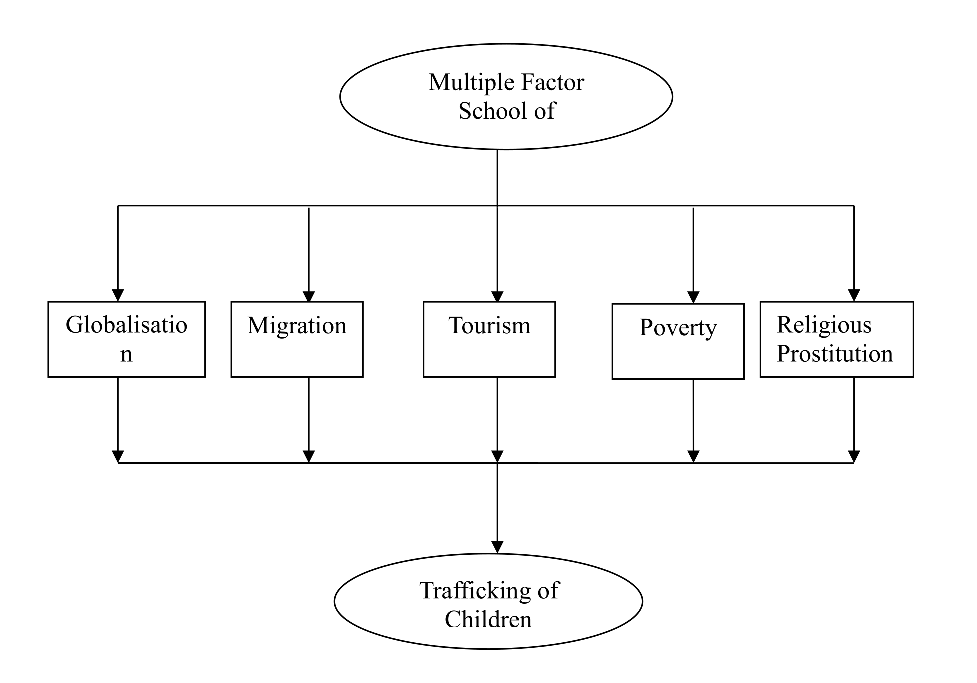
\includegraphics[scale=1.1]{images/fig001.eps}
\end{figure}

\vspace{-.3cm}

\begin{multicols}{2}




\end{multicols}
\label{end2016-art5}
